\section{Materials preparation}

  \subsection{Plasmid construction}

    Plasmids for the canonical histones H2B, H3, and H4,
    respectively pBOS--H2B--GFP, pBOS--H3--EYFP.MC--N1, and pBOS--H4--ECFP.M--N1,
    were provided by Prof. Kevin Sullivan from National University of Ireland,
    Galway. The pBOS--H2B--GFP plasmid has been previously published
    \citep{KevinH2BGFP}. DNA sequencing identified the H3 plasmid as
    the HIST1H3B gene, encoding H3.1 from histone cluster 1; the H4 plasmid
    as either HIST1H4J or HIST1H4K; and the H2B plasmid most similar to the
    HIST1H2BJ gene but with two missense mutations, D25G and V118I.

    Plasmid pPAGFP--N1 and mCherry--\textalpha--tubulin was provided by
    Chelly van Vuuren from National University of Ireland, Galway.

    The HeLa cDNA library was a kind gift by Nadine Quinn from National University
    of Ireland, Galway \citep{NadineThesis}.

    Plasmid pMH3.2--614, which includes a mouse replication dependent histone~H3
    gene, including its upstream and downstream regulatory elements \citep{pMH3-plasmid},
    was provided by Prof. Kevin Sullivan from National University of Ireland, Galway.

    \paragraph{H2B--EGFP}
      The two mutations in the original plasmid were corrected by two
      individual PCR mutagenesis. The first fixed V118I with primers
      AFG112 and AFG113, the second fixed D25G with primers AFG114 and
      AFG115.

    \paragraph{H4--ECFP R45H}
      The R45H mutation was inserted into the pBOS--H4--ECFP.M--N1 by
      PCR mutagenesis using the primers AFG124 and AFG125. The codon
      \texttt{CAC} was selected for the histidine amino acid due to its
      higher codon usage in the human genome\citep{codon_usage}.

    \paragraph{pBOS--GFP}
      A pBOS--GFP vector was prepared from pBOS--H2B--GFP by digestion
      with KpnI and BamHI. The band corresponding to the linearised vector
      without the H2B sequence was purified by gel extraction and used in
      ligation with the H2A sequence.

    \paragraph{H2A--EGFP}
      The H2A sequence was amplified from HeLa genomic DNA with primers
      AFG116 and AFG118. This amplified the coding sequence for the
      HIST1H2AB gene since it has the same sequence used in the previous
      \textit{in vitro} studies that we aim to validate \citep{flaus2004sin}.
      The only other sequence encoding the same protein was HIST1H2AE but has
      a lower codon adaptation index and predicted 5' mRNA secondary
      structures more complex.

    \paragraph{H2AX--EGFP and S139 mutants}
      Closing strategy for cloning the H2AX sequence was similar to the
      strategy for cloning H2A but using the primers AFG130 and AFG131.
      Mutations to H2AX S139, an important site that is phosphorylated during
      DNA damage response,
      was performed at the same time of gene amplification since its location
      is close to the sequence 3' end. The primers AFG132, AFG133, and AFG134,
      were used instead of AFG131 for mutations S139A, S139D, and S139E
      respectively. The mutation to alanine blocks, while
      mutation to aspartic and glutamic acid mimic phosphorylation.
      This strategy introduced an accidental frameshift mutation near the
      stop codon which was fixed by PCR mutagenesis using primers AFG400
      and AFG401.

    \paragraph{H2A.Z--EGFP}
      Unlike the H2A and H2AX plasmids which were prepared from genomic DNA,
      the H2A.Z sequence was amplified from an HeLa cDNA library due
      to the existence of introns in the H2AFZ gene. The amplification PCR
      was performed with primers AFG121 and AFG122. Purification of the
      amplicon and ligation to the pBOS vector was identical to the preparation
      of the H2A--GFP plasmid.

    \paragraph{H4--EYFP}
      The plasmids pBOS--H3--EYFP.MC--N1 and pBOS--H4--ECFP.M--N1 were
      digested with the restriction enzymes BamHI and NotI. After agarose
      gel electrophoresis, the EYFP insert and pBOS--H4 vector were purified
      by gel extraction. The two DNA fragments were ligated to construct
      pBOS-H4-EYFP. The same strategy was used to construct the EYFP tagged
      H4~R45H mutant.

    \paragraph{H3--EYFP T45A and T45E}
      Mutations to H3 T45 were inserted into the pBOS--H3--EYFP.MC--N1 by
      PCR mutagenesis. The primers AFG151 and AFG152 were used for the
      T45E mutation, and AFG153 and AFG154 for T45A.

    \paragraph{H2B and H3 PAGFP}
      The PAGFP insert was prepared from pPAGFP--N1 by PCR using the
      primers AFG478 and AFG479, the amplicon purified by agarose gel
      extraction, digested with NotI and BamHI, and finally cleaned by
      PCR purification.
      Both pBOS--H2B--GFP and pBOS--H3--EYFP.MC--N1 plasmids were also
      digested with NotI and BamHI to excise their tags, and the vectors
      purified by agarose gel extraction. The insert was finally ligated
      into the two vectors for pBOS--H2B--PAGFP and pBOS--H3--PAGFP.
      This strategy introduces a Proline to Arginine mutation in the
      linker for the H2B plasmid.
      %% This mutation in the H2B linker (DPPVAT to DPRVAT) was on purpose.
      %% We could have easily avoid it but would cost us one extra primer
      %% and it shouldn't be making a difference.

    \paragraph{pMH2B--GFP and pMH3--EYFP}
      %% I'm actually not sure if Keving gave me the pMH3.2--614 or the
      %% pCA-TAG plasmid. I did not have any plasmid map or sequence, only
      %% the very small Figure 5 of his paper PMID:9024683
      %% I couldn't even use any standard sequencing primer and by the time
      %% we cloned our genes there, we had already decided to kill the project
      %% so we never got to actually try these in human cells.
      Insertion of the H2B--GFP and H3--EYFP coding sequences into the
      pMH3.2--614 plasmid was performed by PCR amplification, bluent-end
      ligation of both vector and inserts due to the absence of restriction
      sites. pMH3.2--614 was amplified with primers AFG417 and AGF418 which
      create a linear sequence that only ignore the H3.2 coding sequence.
      The H2B--GFP coding sequence was generated with primers AFG419 and AFG420.
      Primers for the insert were phosphorylated by T4~PNK prior to the PCR
      since T4~PNK is more efficient on single stranded DNA. pM vector and
      H2B--GFP insert were purified by agarose gel extraction and ligated.
      Strategy for H3--EYFP was equivalent but using primers AFG424 and AFG420.

  \subsection{Cell lines}

    Transfection was always performed by lipofection~(\Sref{methods:lipofection}),
    both for transient and stable cell lines.

    For creation of stable cell lines, cells were trypsinized and split
    1:20 on \SI{10}{\cm} dishes 24~hours after transfection.
    After another 24 hours, Blasticidin-S was added to the medium for
    a final concentration of \SI{3}{\ug\per\ml} as found by performing a
    Blasticidin-S kill-curve (\Sref{sec:methods:kill-curve}).
    Cell growth was followed and medium replaced when appropriate.
    As cell colonies started to be visible by the naked eye, approximately
    3~weeks after plating, these were screened by fluorescence microscopy.
    Positive colonies were aspirated and moved into 24-well plates with
    \SI{1}{\ml} disposable pipette tips, and the thinnest extremity removed.

    \begin{figure}
      \centering
      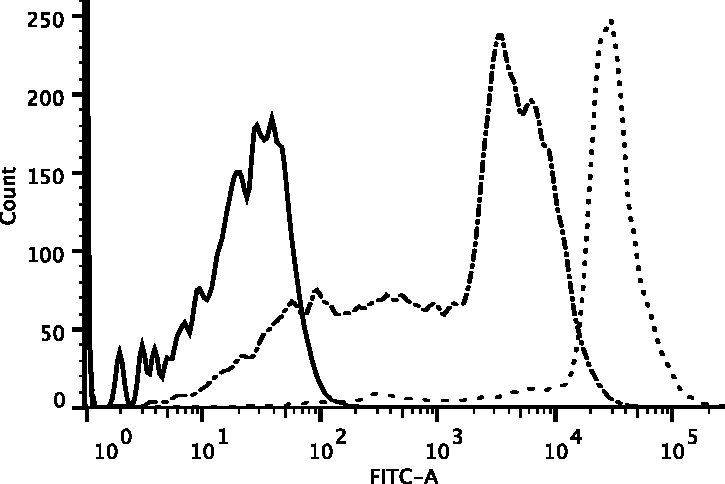
\includegraphics[width=\textwidth]{facs-stable-cell-lines.pdf}
      \captionIntro{FACS sorting of mixed populations}
        {
          The multiple populations with differing intensity values were
          sorted by FACS. The full line represents the intensity profile
          of HeLa wild type cells; the dash-dot line, a mixed population
          of HeLa cells expressing H2B--EGFP; and the dotted line, the
          sorted population.
        }
      \label{fig:methods:facs}
    \end{figure}

    Populations with mixed levels of fluorescent intensity were frequently
    obtained while preparing stable cell lines. In such cases, cells with
    similar intensity of their corresponding fluorophore were FACS
    sorted (\fref{fig:methods:facs}).

    The following stable lines were prepared:

    \begin{itemize}
      \item HeLa H2B--EGFP
      \item HeLa H2B--EGFP D25G V118I
      \item HeLa H3--EYFP
      \item HeLa H3--EYFP T45A
      \item HeLa H3--EYFP T45E
      \item HeLa H4--EYFP
      \item HeLa H4--EYFP R45H
    \end{itemize}

  \subsection{Microscopy}

    Both stable and transiently cell lines were used in imaging. When
    transiently transfected cells were being used, transfection was performed
    approximately 48~hours before imaging.

    Confocal microscopy was performed with a Zeiss LSM510 Meta microscope
    using glass bottom LabTek II chambers. Wide-field fluorescence microscopy
    was performed with an Applied Precision DeltaVision Core system
    using \SI{35}{\mm} glass bottom MatTek dishes.

    In both cases, imaging was performed within an acrylic environmental
    chamber that fully enclosed the stage plate and microscope objectives.
    Temperature and CO$_2$ levels were maintained via separate units connected
    to the environmental chamber.

  \subsection{Computational analysis}

    Software used for image analysis and visualization was described in
    \Sref{sec:methods:software}

    Original source code written in \textsc{Matlab} for a previously
    reported circle FRAP model \citep{mueller2008evidence} was kindly offered
    to us under the GNU General Public License (GPL) version~3 by the
    original authors. A port of this code for the GNU Octave language was
    prepared and made available under the same license.

